% Copyright 2004 by Till Tantau <tantau@users.sourceforge.net>.
%
% In principle, this file can be redistributed and/or modified under
% the terms of the GNU Public License, version 2.
%
% However, this file is supposed to be a template to be modified
% for your own needs. For this reason, if you use this file as a
% template and not specifically distribute it as part of a another
% package/program, I grant the extra permission to freely copy and
% modify this file as you see fit and even to delete this copyright
% notice. 

\documentclass[handout]{beamer}
\usepackage{blindtext}
\usepackage{graphicx}
\usepackage{subfiles}
\usepackage{amsmath}
\usepackage{amsthm}
\usepackage{tikz}
\usepackage{wrapfig}
\usepackage{lscape}
\usepackage{rotating}
\usepackage{epstopdf}
\usepackage{subcaption}
\usepackage[font=small,labelfont=bf]{caption}
\usepackage{hyperref}
\usepackage{color}
\usepackage{verbatim}
\usepackage{algorithm}% http://ctan.org/pkg/algorithms
\usepackage{algpseudocode}% http://ctan.org/pkg/algorithmicx
\usetikzlibrary{shapes.geometric, arrows}
\theoremstyle{definition}
\theoremstyle{remark}
\newtheorem*{remark}{Remark}
\usepackage{amssymb}
\usepackage{amsfonts}
\usepackage{mathtools}
\newcommand{\defeq}{\vcentcolon=}
\newcommand{\eqdef}{=\vcentcolon}
\newcommand*{\V}[1]{\mathbf{#1}}%
\newcommand{\norm}[1]{\left\lVert#1\right\rVert}
\newcommand{\justif}[2]{&{#1}&\text{#2}}
\newcommand{\qedwhite}{\hfill \ensuremath{\Box}}
\newcommand\given[1][]{\:#1\vert\:}
\newcommand{\me}{\mathrm{e}}
\DeclarePairedDelimiterX{\infdivx}[2]{(}{)}{%
  #1\;\delimsize\|\;#2%
}
\DeclarePairedDelimiter\abs{\lvert}{\rvert}%
\newcommand{\Conv}{\mathop{\scalebox{1.5}{\raisebox{-0.2ex}{$\ast$}}}}%
\newcommand{\infdiv}{\infdivx}
\newcommand{\parder}[2]{\frac{\partial{#1}}{\partial{#2}}}
\renewcommand{\qed}{\hfill\blacksquare}

% There are many different themes available for Beamer. A comprehensive
% list with examples is given here:
% http://deic.uab.es/~iblanes/beamer_gallery/index_by_theme.html
% You can uncomment the themes below if you would like to use a different
% one:
%\usetheme{AnnArbor}
%\usetheme{Antibes}
%\usetheme{Bergen}
%\usetheme{Berkeley}
%\usetheme{Berlin}
%\usetheme{Boadilla}
%\usetheme{boxes}
%\usetheme{CambridgeUS}
%\usetheme{Copenhagen}
%\usetheme{Darmstadt}
%\usetheme{default}
%\usetheme{Frankfurt}
%\usetheme{Goettingen}
%\usetheme{Hannover}
%\usetheme{Ilmenau}
%\usetheme{JuanLesPins}
%\usetheme{Luebeck}
\usetheme{Madrid}
%\usetheme{Malmoe}
%\usetheme{Marburg}
%\usetheme{Montpellier}
%\usetheme{PaloAlto}
%\usetheme{Pittsburgh}
%\usetheme{Rochester}
%\usetheme{Singapore}
%\usetheme{Szeged}
%\usetheme{Warsaw}

\title{The path to LSTMs}

% A subtitle is optional and this may be deleted
\subtitle{A succinct introduction}

\author{Bernardo P\'erez Orozco \\ \href{mailto:ber@robots.ox.ac.uk}{ber@robots.ox.ac.uk} }
% - Give the names in the same order as the appear in the paper.
% - Use the \inst{?} command only if the authors have different
%   affiliation.

\institute[University of Oxford] % (optional, but mostly needed)
{
  Department of Engineering Sciences\\
  University of Oxford}
% - Use the \inst command only if there are several affiliations.
% - Keep it simple, no one is interested in your street address.

\date{MLRG Tea Talk Series, 2016}
% - Either use conference name or its abbreviation.
% - Not really informative to the audience, more for people (including
%   yourself) who are reading the slides online

\subject{Machine Learning}
% This is only inserted into the PDF information catalog. Can be left
% out. 

% If you have a file called "university-logo-filename.xxx", where xxx
% is a graphic format that can be processed by latex or pdflatex,
% resp., then you can add a logo as follows:

% \pgfdeclareimage[height=0.5cm]{university-logo}{university-logo-filename}
% \logo{\pgfuseimage{university-logo}}

% Delete this, if you do not want the table of contents to pop up at
% the beginning of each subsection:
\AtBeginSubsection[]
{
  \begin{frame}<beamer>{Outline}
    \tableofcontents[currentsection,currentsubsection]
  \end{frame}
}

% Let's get started
\begin{document}

\begin{frame}
  \titlepage
\end{frame}



% Section and subsections will appear in the presentation overview
% and table of contents.
\section*{Introduction}

\begin{frame}{Introduction}
  \begin{itemize}
      \item{ Deep Learning revolution: neural networks (NN) \pause
      \begin{itemize}
          \item ``Deep'' models = ``many'' layers \pause
      \end{itemize}
      }
      \item LSTM is state-of-the-art in sequence learning \pause
      \item LSTM is a specific case of Recurrent NNs (RNNs) \pause
      \item LSTM exists because: \pause
      \begin{itemize}
          \item NNs are most often trained by gradient descent... \pause
          \item ... and you can't train general RNNs by gradient descent!
      \end{itemize}
  \end{itemize}
\end{frame}

\begin{frame}{Outline}
  \tableofcontents
  % You might wish to add the option [pausesections]
\end{frame}

\section{Building a path to LSTMs}

\subsection{A review of Neural Networks}

\begin{frame}{Neural networks}
  \begin{itemize}
  \item{
    A NN is a collection of mappings called \textbf{layers}
    \pause
  }
  
  \item{
    Each layer contains a number of \textbf{neurons} (hidden units) 
    \pause
  }
  
  \item{
    Neurons are feature detectors, i.e. they react to stimuli 
    \pause
  }
  
  \item{
    \textbf{Example:} Dense unit outputs $h = \phi(\V{w}^T\V{x} + b)$, where $\phi$ is called the activation function of the unit.
    \pause
  }
  \end{itemize}
  
  \centering
  
\includegraphics[width=5cm]{figs/neuron.png}
  
\end{frame}

\begin{frame}{Neural Networks}{Neurons and layers}
  \begin{itemize}
      \item We don't \textbf{think of NNs} in terms of neurons, but rather \textbf{in terms of layers} with parameters $\theta$: \pause
  \end{itemize}
  
  \centering
  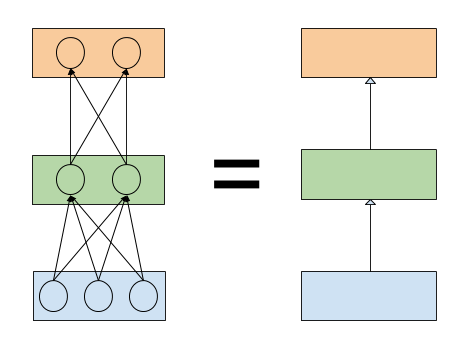
\includegraphics[width=5cm]{figs/mlp.png}
\end{frame}


\begin{frame}{Feedforward NNs}{Dense layer}
  \begin{block}{Dense layer}
   A dense layer is a mapping $H:\mathbb{R}^n \rightarrow \mathbb{R}^m$ given by $H(\V{x}) = \phi(\V{Wx}+\V{b})$, where:
   
   \begin{itemize}
       \item $\V{x}$ is the input to the layer
       \item $\V{h} = H(\V{x})$ are the output or activations
       \item $\phi$ is called activation function
       \item $m$ is number of neurons in the layer
       \item $\theta = (\V{W, b})$ are the parameters of the layer 
   \end{itemize}
  \end{block}
  \begin{itemize}
      \item Output $\V{h}$ indicates \alert{amount of activity} in the neuron
  \end{itemize}
\end{frame}

\begin{frame}{Feedforward neural networks}{Activation functions}
\begin{itemize}
    \item Some common activation functions are:
  \begin{align*}
    \sigma(x) &= \frac{1}{1+e^{-x}}\\
    \text{tanh}(x) &= \frac{e^x - e^{-x}}{e^x + e^{-x}}\\
    \text{ReLU}(x) &= \max(0, x)
  \end{align*}
  
   
\end{itemize}
  
\end{frame}

\subsection{Deep Learning}

\begin{frame}{Deep learning}
\begin{itemize}
    \item{
        Models have ``many'' layers \pause
        \begin{itemize}
          \item Convolutional networks \pause
          \item Recurrent networks \pause
          \item Autoencoders \pause 
        \end{itemize}
    }
    \item{
        Advances in optimisation \pause
        \begin{itemize}
          \item Developments in gradient descent \pause
          \item New regularisation techniques, e.g. dropout \pause
        \end{itemize}
    }
    \item{
        Why is depth important?
        \begin{itemize}
            \item{ Lower layers detect simple features, e.g. edges \pause }
            \item{ Upper layers learn complex features by combining simpler ones, e.g. combine edges to get shapes \pause }
        \end{itemize}
    }
    
    \item{ Why now?
        \begin{itemize}
            \item{ DL has been around since the 80s! \pause}
            \item{ Better hardware: GPUs \pause}
            \item{ Better software: specialised libraries}
        \end{itemize}
    }
\end{itemize}  
\end{frame}

\subsection{Gradient descent developments}
\begin{frame}{Gradient descent developments}{Vanilla gradient descent}
  \begin{block}{Gradient descent}
  Iterative optimisation method. Update rule is given by:
  \begin{align*}
      \theta_{t+1} = \theta_t - \alpha\nabla_\theta L(\theta)
  \end{align*}
  \begin{itemize}
      \item Learning rate: $\alpha$
      \item Loss function or criterion: $L(\theta)$
  \end{itemize} 
  \end{block} 
\end{frame}

\begin{frame}{Gradient descent developments}{Recent developments}
  \begin{itemize}
      \item { Stochastic minibatch gradient descent \pause 
        \begin{itemize}
          \item Approximate gradient over random minibatch for multiple updates per epoch \pause
        \end{itemize}
      }
      \item{ Adaptive methods \pause
        \begin{itemize}
          \item Learning rate changes with time \pause
        \end{itemize}
      }
      \item {Momentum \pause
        \begin{itemize}
          \item New updates consider previous updates, i.e. gain momentum on descent\pause
        \end{itemize}
      }
      \item{
        AutoDiff \pause
        \begin{itemize}
          \item Program $P$ computes $f(\theta)$. AutoDiff finds program $P'$ that computes $\nabla_\theta f(\theta)$ efficiently.
        \end{itemize}
      }
      \item{
        Examples: Adam, RMSprop, Adadelta
      }
  \end{itemize}
\end{frame}


\subsection{Recurrent Neural Networks}

\begin{frame}{Recurrent Neural Networks}
  \begin{block}{The RNN layer}
  The recurrent neural network layer is given by:
  \begin{align*}
      \V{h}_t = \V{W_r}\phi(\V{h_{t-1}}) + \V{W_ix}_t + \V{b}
  \end{align*}
  with $\theta = (\V{W}_i, \V{W}_r, \V{b})$
  \end{block}
  
  \begin{itemize}
      \item{ From the equation above, it is easy to see that $\V{h}_t = f(\V{h}_{t-1}, \V{x}_t, \theta)$, and furthermore $\V{h}_t = f(f(...f(\V{h}_0, \V{x}_1, \theta)..., \V{x}_{t-1}, \theta), \V{x}_t, \theta)$, where $\V{h}_0$ is the initial state of the recurrent network. \pause}
  \end{itemize}
\end{frame}

\begin{frame}{Recurrent Neural Networks}{Unfolding the network}
  \centering
  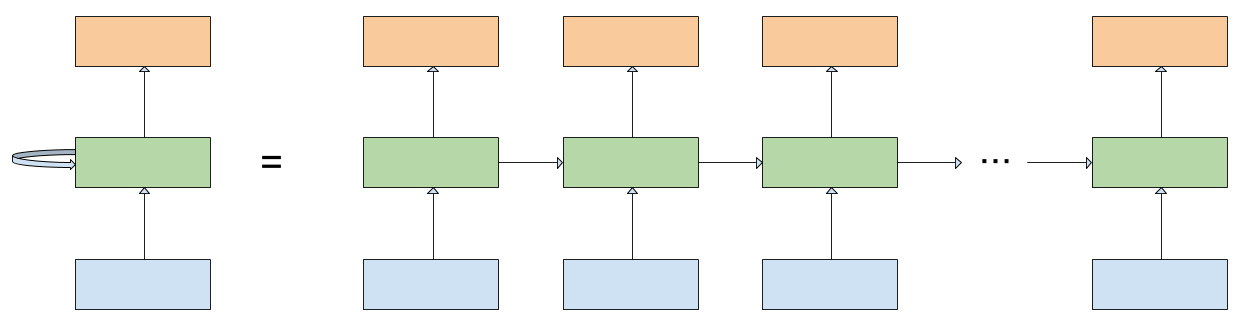
\includegraphics[width=12cm]{figs/rnn.png}
\end{frame}

\begin{frame}{Recurrent Neural Networks}{Problems with the gradient}
  \begin{itemize}
      \item {Compute gradient to train by gradient descent\pause}
      \begin{align*}
          &\frac{\partial\V{h}_t}{\partial\theta_j} = \frac{\partial\V{W}_r}{\partial\theta_j} \phi(\V{h_{t-1}}) + \V{W}_r\frac{\partial \phi(\V{h}_{t-1})}{\partial\V{h}_{t-1}}\frac{\partial \V{h}_{t-1}}{\partial\theta_j}\\
    &= \frac{\partial\V{W}_r}{\partial\theta_j} \phi(\V{h_{t-1}}) + \V{W}_r\phi'(\V{h}_{t-1})\frac{\partial \V{h}_{t-1}}{\partial\theta_j}\\
    &= \frac{\partial\V{W}_r}{\partial\theta_j} \phi(\V{h_{t-1}}) + \alert{\V{W}_r\phi'(\V{h}_{t-1})}\left(\frac{\partial\V{W}_r}{\partial\theta_j} \phi(\V{h_{t-2}}) + \alert{\V{W}_r\phi'(\V{h}_{t-2})}\frac{\partial \V{h}_{t-2}}{\partial\theta_j}\right)
      \end{align*}
  \end{itemize}
\end{frame}

\begin{frame}{Recurrent Neural Networks}{Problems with the gradient}
  \begin{itemize}
      \item{Exploding gradient\pause
        \begin{itemize}
            \item{Can be handled by heuristics, e.g. gradient clipping\pause}
        \end{itemize}
      }
      \item{Vanishing gradient\pause
        \begin{itemize}
            \item{Currently solved by means of architectural changes, i.e. LSTM\pause}
        \end{itemize}
      }
      
  \end{itemize}
\end{frame}


\section{The LSTM architecture}

\subsection{The LSTM layer}

\begin{frame}{The LSTM layer}
  \begin{block}{The LSTM layer}
  The LSTM layer directly addresses the issue of the vanishing gradient by means of a gating mechanism, and is given by the following equations\footnotemark:
\begin{align*}
    \V{x}'_t &= [ \V{x}_t, \V{h}_{t-1} ]\\
    \V{S}_t &= \tanh(\V{W}_S\V{x}'_t + \V{b}_S)\\
    \V{C}_t &= \V{i}_t\odot\V{S}_t + \V{f}_t\odot\V{C}_{t-1}\\
    \V{h}_t &= \V{o}_t \odot \tanh(\V{C}_t)
\end{align*}
\par where $\V{i}_t, \V{o}_t, \V{f}_t$ are called the input, output and forget gates given by:
\begin{align*}
    \V{i}_t &= \sigma(\V{W}_i\V{x}'_t + \V{b}_i)\\
    \V{o}_t &= \sigma(\V{W}_o\V{x}'_t + \V{b}_o)\\
    \V{f}_t &= \sigma(\V{W}_f\V{x}'_t + \V{b}_f)
\end{align*}
  \end{block}
  \footnotetext[1]{Where $\V{x}\odot\V{y}$ refers to the element-wise product of vectors $\V{x}, \V{y}$.}
\end{frame}

\begin{frame}{The LSTM layer}
  \begin{itemize}
      \item {We call $\V{C}_t$ the \textit{memory cell} at time $t$, and it is arguably the main component of the LSTM architecture.\pause}
      \item{We can think of the LSTM in the following manner:
      \begin{align*}
    \V{C}_t &= \V{i}_t\odot\V{S}_t + \V{f}_t\odot\V{C}_{t-1}\\
    \text{memory}_t &= \text{read}\odot\text{input}_t + \text{remember}\odot\text{memory}_{t-1}
\end{align*}
      \pause}
  \end{itemize}
\end{frame}

\begin{frame}{The LSTM layer}{Why does it work?}
  \begin{itemize}
      \item {Similar reasoning: \pause
      \begin{align*}
    \parder{\V{h}_t}{\theta_j} &= \parder{\V{o}_t}{\theta_j}\odot\tanh(\V{C}_t) + \V{o}_t\odot\parder{\tanh(\V{C}_t)}{\V{C}_t}\parder{\V{C}_t}{\theta_j}\\
    \parder{\V{C}_t}{\theta_j} &= \parder{\V{i}_t}{\theta_j}\odot\V{S}_t +  \V{i}_t\odot\parder{\V{S}_t}{\theta_j} + \parder{\V{f}_t}{\theta_j}\odot\V{C}_{t-1} + \V{f}_t\odot\parder{\V{C}_{t-1}}{\theta_j}
\end{align*} \pause
    }
    
    \item{The term $\parder{\V{C}_t}{\theta_j}$ is also a function of $\parder{\V{C}_{t-1}}{\theta_j}$\pause
    \begin{itemize}
        \item {$\V{C}_{t-1}$ does not go through non-linear $\phi$\pause}
        \item{Weighted by the element-wise product of the previous $k$ forget gates $\prod_{T=k}^t\V{f}_T$. The LSTM can only forget once $\V{f}_k$ tends to zero.}
    \end{itemize}
    }
  \end{itemize}
\end{frame}

\subsection{LSTM applications and other work}
\begin{frame}{LSTM applications}
  \begin{itemize}
      \item Speech recognition \pause
      \item Sequence generation (handwriting and Shakespeare texts) \pause
      \item Financial forecasting \pause
      \item Reinforcement learning \pause
      \item Models of attention (scene labelling) \pause
      \item Check reading list in notes!
  \end{itemize}
\end{frame}

\section{Keras}
\begin{frame}{Keras}{Why Keras?}
  \begin{itemize}
      \item Integrates routines for: training, testing, data preprocessing, activation, regularisation and loss functions, and optimisation procedures. \pause
      \item Inherits AutoDiff, GPU compatibility from Theano/TensorFlow (backends). \pause
      \item Paradigm: stack modules (Torch-like) \pause
      \item Well documented \pause 
      \item Runs on Python
  \end{itemize}
\end{frame}

\begin{frame}{Keras}{Work pipeline}
  \begin{enumerate}
      \item Prepare data: xTrain, yTrain, xTest, yTest \pause
      \item Init empty layer: model = Sequential() \pause
      \item Stack layers: model.add(...) \pause
      \item Compile model: model.compile( loss, optimiser )\pause
      \item Train: model.fit( xTrain, yTrain, ... ) \pause
      \item Test: model.predict( xTest ) 
  \end{enumerate}
\end{frame}

\section{Opportunities and future work}
\begin{frame}{Open questions}
  \begin{itemize}
      \item{ No probabilistic reasoning \pause
        \begin{itemize}
            \item Measuring uncertainty? \pause
            \item Variational methods? \pause
        \end{itemize}
      }
      \item{
        Little interpretability \pause
        \begin{itemize}
            \item What do its hidden representations mean? \pause
        \end{itemize}
      }
      \item{
        Most applications are classification problems
        \begin{itemize}
            \item More time series forecasting! 
        \end{itemize}
      }
  \end{itemize}
\end{frame}

\end{document}


